\documentclass[11pt]{article}
\usepackage{graphicx}
\usepackage{enumitem}
\usepackage{amsmath}
\usepackage{hyperref}
\begin{document}

\section{Implementation}
In this section we present our implementation of LDA in \textit{Python} and discuss our results on real data. 
\subsection{Library Used}
	
    \begin{itemize}[noitemsep]
		\item \textit{scikit learn}  for pre-processing.
		\item \textit{scipy} for probability distributions.
 	\end{itemize}
\subsection{Dataset Description}
The dataset used is the same one used in the authors implementation. it can be found at the following link: \texttt{ https://nlp.stanford.edu/software/tmt/tmt-0.4/}
It consist of 2246 small documents. We used 2000 documents for training our model and kept the rest for testing (classification).
   
\subsection{Pre-processing}
\textbf{Tokenization of the documents:}  LDA uses the bag of word assumption (the order of words apparitions in a document is ignored). This allows us to use a compact representation of documents in a matrix of M x V.  Each line in the matrix represents a document and the values are integer that represent the number of occurrences of a word in the vocabulary. This is similar to the one hot encoding trick that we used in the class. \\
\\
In addition  to tokenization, we included the following filters: 
    \begin{itemize}[noitemsep]
   	    \item Removed non-alphabetical characters.
		\item Removed words with only 1 occurrence across the corpus.
		\item Removed words that occur in 95 \%  or more of the documents. 
	\end{itemize}
Finally, Due to the limited memory of our hardware and for runtime reasons, we limited the vocabulary to only the 3000 most frequent words of the corpus. 

\subsection{Hyperparameter Selection}
We chose our topic vector $\alpha$ to be of size 100 to match the original implementation of the author. 

\subsection{Parameter   Initialization}
As stated in section xxxx, LDA with with variational EM has 4 sets of parameters to estimate. The parameters initialized to the following value:

\begin{tabular}{ |p{2cm}||p{3cm}|p{10cm}| }
 \hline
 Parameter & Dimension  & Initialization\\
 \hline
  $\alpha$& [K]   & np.random.gamma(shape=np.ones((K)), scale=1/K)\\
  $\beta$  & [K x V]  &  np.random.dirichlet(np.ones(V), K)\\
  $\gamma $  & [M x K]  &  alpha + (N[d] / K)  \\
  $\phi$  & [M x N[d] x K]  &   np.ones((N[d], K))/ K \\
  \hline
\end{tabular}\\
\\
\\
\subsection{Stopping Criteria }
In the paper, the author doesn't state very clearly the stopping criterion used in its implementation. So we chose to stop the model once the parameter L2 norm of $\gamma$   from one iteration to the next is is below a given threshold. 
\\

\begin{figure}[ht]
\vskip 0.2in
\begin{center}
\centerline{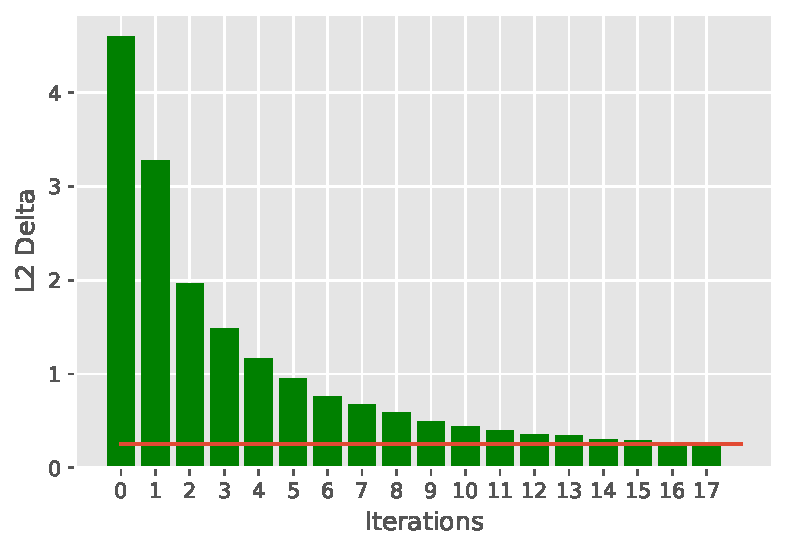
\includegraphics[width=\columnwidth]{plot_delta_gamma_convergence}}
\caption{Change in $\gamma$ parameter across EM iterations. The green bars represent the L2 change of  $\gamma$ parameters. The red line represent the stopping criterion  used (0.25 in our case).}
\label{icml-historical}
\end{center}
\vskip -0.2in
\end{figure}

\section{Empirical Results}
\subsection{Topic Extraction}
The canonical use of topic modeling is to find a list of topics across a corpus of text. We can attempt to understand the meaning of a topic using the words with the highest probability for the given topic. %$\argmax_{ p(\beta \mid \alpha)}$
\begin{table}[h]
\caption{Topic Sample from LDA model: each column represents the top 10 words from the topic. We can see that the topics are easy to interpret. for full list of topic, see: }%Topics_list.csv

  \scalebox{0.6}{
    \begin{tabular}
    { |p{2cm}|p{2cm}|p{2.5cm}|p{2cm}|p{2cm}| }
 \hline
 \multicolumn{5}{|c|}{Topic Sample} \\
 \hline
 Topic 1: & Topic 2:   &  Topic 3: & Topic 4:  & Topic 5: \\
   Politics & Finance & Trial  & Crime & Korea\\
 \hline
 trade & york & years & authorities & roh\\
 committee & shares & guilty & city & hostages\\
 senate & board & case & injured & guard\\
 new & million & trial & shot & officials\\
 time & exchange & prison & hospital & coast\\
 abortion & trading & said & night & korean\\
 bush & stocks & judge & killed & korea\\
 president & index & court & people & south\\
 souter & market & attorney & police & north\\
 said & stock & charges & said & said\\
 \hline
\end{tabular}}
\end{table}

\subsection{Document Classification}
LDA can also be used to classify previously unseen document to one of the K-topics. First, we need to perform variational inference on the unseen document and use the trained gamma parameter to assign the document to the most likely topic. We scored the holdout documents and made a manual comparison of document vs topics. Overal, the topic made sense. See table 2 for a sample of document.  Full results of the test set can be found in the following file: \begin{verbatim}
classification_holdout.csv 
\end{verbatim}


\hyperref{ https://nlp.stanford.edu/software/tmt/tmt-0.4/}
\end{document}
